\documentclass{article}
\usepackage[utf8]{inputenc}
\usepackage[portuguese]{babel}
\usepackage{graphicx}
\usepackage{hyperref}
\usepackage{float}

\hypersetup{
    colorlinks=true,
    linkcolor=blue,
    filecolor=magenta,      
    urlcolor=cyan,
}


\title{Trabalho 3 - Redes de Computadores I}
\author{Gustavo Kundlatsch (17102810)}
\date{\today}

\begin{document}

\maketitle

\begin{abstract}
    O objetivo desse trabalho é obter conhecimentos práticos no uso do software Wireshark, que analisa o tráfego de rede, e o organiza de acordo com protocolos, IPs envolvidos ou diversos outros filtros que o usuário pode selecionar. Através desse aplicativo podemos controlar o tráfego de uma rede e monitorar a entrada e saída de dados do computador, através de diversos protocolos, ou a entrada e saída de dados da rede à qual o computador está ligado.
\end{abstract}{}

\section{Introdução}

Nesse trabalho vamos utilizar o software Wireshark para identificar pacotes realizando conexões, transferência de dados e a desconexão, analisando as camadas de aplicação, rede e transporte. Os pacotes analisados na demonstração utilizaram o protocolo TCP e HTTP. O trabalho foi realizado utilizando um computador pessoal, com um processador Intel(R) Core(TM) i7-6500U CPU @ 2.50GHz, 8GB de memória RAM DDR3 e uma placa de vídeo NVIDIA GeForce 930M. A rede em que o computador estava conectado era a rede pessoal, de uma república (uma casa contendo seis estudantes, com diversos dispositivos cada, como computadores, notebooks, celulares e tablets).

\section{Funcionamento}

\subsection{Conexão}

No processo de estabelecer uma conexão, o objetivo normalmente é estabelecer uma ligação entre o usuário final e o servidor. O primeiro passo para isso acontecer é o usuário enviar um pacote TCP com a flag [SYN], com o objetivo de estabelecer a conexão. Caso o servidor possa aceitar a conexão, ele irá responder com um pacote com a flag [SYN, ACK] para satisfazer a mensagem anterior. Quando o usuário recebe esse pacote, ele reponde com um pacote [ACK] para satisfazer a mensagem do servidor. Se todos os passos funcionarem, a conexão será bem estabelecida.

\subsection{Transferência de Dados}

Para explicar o funcionamento da transferência de dados, vamos conceituar algumas coisas primeiro. TCP/IP é um conjunto de protocolos. Diferente do formato OSI que é dividido em sete camadas, os protocolos TCP/IP está equivalentemente organizado em quatro camadas apenas. Quando dois programas se comunicam através da internet, por exemplo, eles estão em contato direto com a primeira camada TCP/IP: Aplicação (mesmo nome da primeira camada OSI).

Nessa camada de aplicação, existem diversos protocolos com diversos objetivos. O foco desse trabalho é explorar a troca de dados HTTP (Hypertext Transfer Protocol). Todo protocolo é criado com o objetivo de padronizar algo que pode ser feito de diversas maneiras. No caso do HTTP, o objetivo é padronizar a transferência de hypermídia, como textos, imagens e sons. Conceitualmente, o hipertexto é uma ligação cujo objetivo é facilitar a navegação dos usuários, através de um texto que pode ser composto de diversas palavras, imagens ou até mesmo sons que, ao serem clicados, direcionam o usuário para outra página onde se esclarece com mais precisão o assunto do link abordado.

Depois de ocorrer o processamento dessa requisição, a camada de aplicação chama a camada de transporte através da porta 80 (esse valor é específico do protocolo HTTP, cada protocolo possui uma porta própria), indicando que tipo de conteúdo será enviado. Em seguida, a camada de transporte deve dividir os dados em pacotes e ordená-los. É aqui que acontece o uso do TCP (Transmission Control Protocol), que tem como objetivo encapsular as informações de controle da seguinte maneira: número da porta de origem, número da porta destino, número de sequência (Seq), soma de verificação (ACK). Após ser encapsulado em forma de cabeçalho de acordo com o TCP, a camada Internet adere os endereços IPs da origem e destino do pacote, para finalmente os pacotes saírem para a Interface com a Rede. Essa camada depende do tipo de rede em que o computador está conectado. É muito comum a rede ser do tipo Ethernet, que adiciona dados no começo dos pacotes e finalmente os convertem em impulsos elétricos.



\subsection{Desconexão}

Quando ou o usuário final ou o servidor querer terminar a conexão, ele deve enviar um pacote TCP com a flag [FIN, ACK]. Caso nenhum erro aconteça, a contra parte irá devolver uma confirmação com uma flag [ACK] num pacote TCP e, então, deve enviar o seu próprio pacote com a flag [FIN, ACK] e esperar a resposta [ACK] correspondente.

\section{Experimento}

Nessa seção vamos desenvolver como foram realizados os experimentos (testes) com o Wireshark para estudar o funcionamento das operações descritas na seção anterior. Para o desenvolvimento do experimento, foi utilizado o site \href{http://wombocombo.com.br/}{http://wombocombo.com.br/}, um blog de notícias de e-sports, que não utiliza SSL (protocolo HTTPS), permitindo visualizar os pacotes. 

\subsection{Conexão}

A conexão é dividida nas três etapas anteriormente descritas. Nas imagens abaixo, as legendas descrevem o processo que está sendo realizado/analisado em cada momento.

\begin{figure}[h]
    \centering
    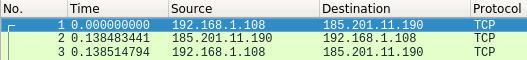
\includegraphics[width=0.9\textwidth]{images/conect1.png}
    \caption{Aqui mostramos os IPs que estão se conectando, e o protocolo que está sendo utilizado}
    \label{fig:conect1}
\end{figure}{}

\begin{figure}[h]
    \centering
    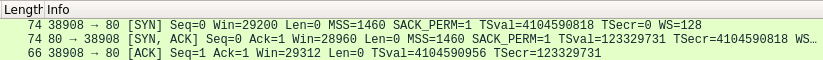
\includegraphics[width=\textwidth]{images/conect2.png}
    \caption{Informações das operações, mostrando o funcionamento de cada uma das etapas, com as flags [SYN], [SYN, ACK] e [ACK] aparecendo em ordem}
    \label{fig:conect2}
\end{figure}{}

\begin{figure}[h]
    \centering
    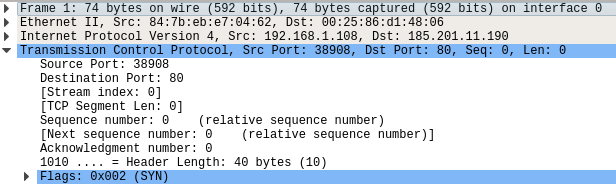
\includegraphics[width=\textwidth]{images/conect3.png}
    \caption{Aqui temos o primeiro pacote aberto, e temos um TCP saíndo do computador indo para o servidor. O pacote leva a flag SYN. Depois disso, é esperado que o servidor responda com as flags SYN, ACK, sendo que o ACK deve ser igual ao SYN do pacote 1, ou seja, `1'. A porta de destino é 80, como esperado, pois o esperado é um HTTP.}
    \label{fig:conect3}
\end{figure}{}

\begin{figure}[h]
    \centering
    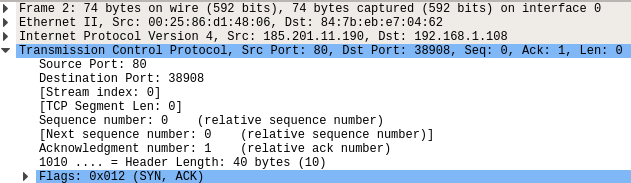
\includegraphics[width=\textwidth]{images/conect4.png}
    \caption{O pacote 2 é a resposta do servidor dizendo o esperado. Tudo que resta é enviar um pacote para o servidor com ACK igual ao do pacote 15, ou seja, `1'.}
    \label{fig:conect4}
\end{figure}{}

\begin{figure}[h]
    \centering
    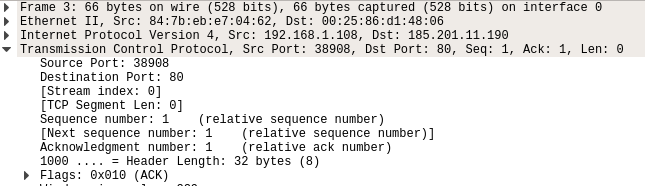
\includegraphics[width=\textwidth]{images/conect5.png}
    \caption{Por fim temos o resultado esperado: ACK = 1, SEQ = 1. A conexão foi bem sucedida.}
    \label{fig:conect5}
\end{figure}{}

\newpage

\subsection{Transferência de Dados}

\begin{figure}[H]
    \centering
    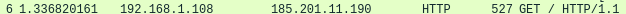
\includegraphics[width=\textwidth]{images/conect6.png}
    \caption{Essa linha é um pedido do computador para que o servidor forneça a página acessada (homepage).}
    \label{fig:conect6}
\end{figure}{}

\begin{figure}[H]
    \centering
    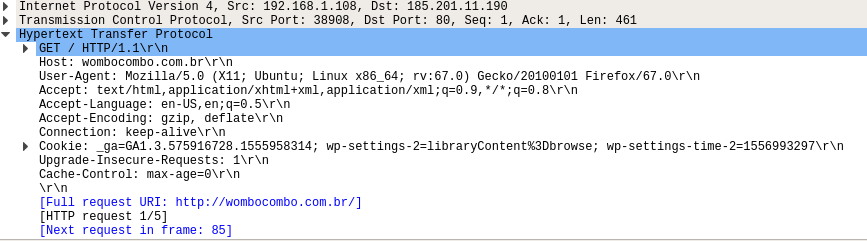
\includegraphics[width=\textwidth]{images/conect7.png}
    \caption{Esta imagem mostra os detalhes do pacote, mostrando o método GET. Ao lado de get aparece uma barra, porque o endereço acessado foi a homepage do site. Caso fosse outra página, haveria o caminho até ela. Depois da barra, aparece a versão do protocolo, nesse caso 1.1.}
    \label{fig:conect7}
\end{figure}{}

\begin{figure}[H]
    \centering
    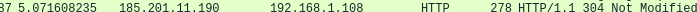
\includegraphics[width=\textwidth]{images/data1.png}
    \caption{O servidor pode ter diversas respostas, o código 200, por exemplo, é o código de sucesso. Nesse caso, o retorno foi um código que significa ``Não alterado''. Esse código serve para motivos de cache, ou seja, a versão da última solicitação do mesmo tipo não sofreu mudanças, então a versão em cache pode ser reaproveitada. Isso acontece pois esse é um site que é frequentemente visitado no computador utilizado para o experimento, ou seja, a versão mais recento do site já estava em chache.}
    \label{fig:data1}
\end{figure}{}

\begin{figure}[H]
    \centering
    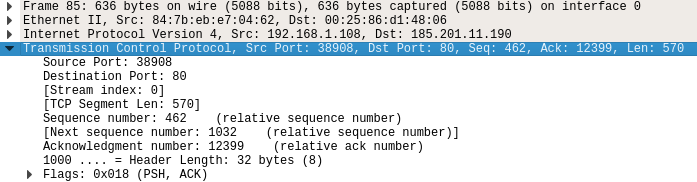
\includegraphics[width=\textwidth]{images/data2.png}
    \caption{Aqui vemos mais informações do pacote, como portas de origem e destino, e o número de sequência e o próximo número de sequência. Esse tipo de informação é mais ou menos relevante de acordo com o tipo da aplicação que está transmitindo. No caso de um servidor de um site de streaming de vídeo, por exemplo, o número de sequência e o próximo número de sequência se tornam bastante relevantes para manter a consistência do vídeo que está sendo transmitido.}
    \label{fig:data2}
\end{figure}{}


\subsection{Desconexão}

\begin{figure}[H]
    \centering
    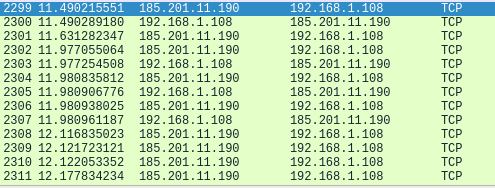
\includegraphics[width=\textwidth]{images/disconectA.png}
    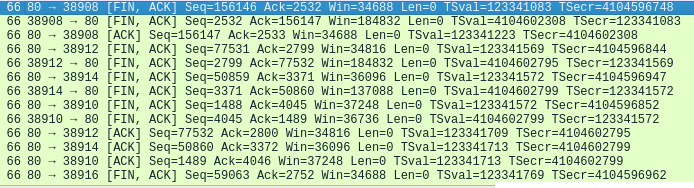
\includegraphics[width=\textwidth]{images/disconectB.png}
    \caption{Nestas duas imagem, que são uma complemento da outra (a primeira ficaria do lado esquerdo, e a segunda no direito, na visualização do Wireshark) temos uma série de pedidos de desconexão. Como foi explicado anteriormente, quem quiser fazer a desconexão (nesse caso o servidor) envia um pacote TCP com a flag [FIN/ACK]. Como não ocorreu nenhum erro, a contra parte (computador) devolveu uma confirmação com uma flag [ACK] num pacote TCP (pacote 2301) e, então, deve enviou o seu próprio pacote com a flag [FIN/ACK], que teve como resposta um pacote [ACK] do servidor, confirmando a desconexão.}
    \label{fig:data2}
\end{figure}{}

\section{Conclusão}

Ao decorrer do experimento, foi possível aprender na prática conceitos que haviam sido trabalhados em sala de aula, de maneira bastante direta e que pode render várias visões de como a rede funciona na vida real. Durante a análise da terceira etapa do experimento, a desconexão, houveram alguns problemas em identificar quais pacotes estavam fazendo quais operações, devido a distância entre a última ação (a transferência de dados) e a desconexão, além de várias desconexões aparentemente estarem ocorrendo juntas. Tirando isso, foi possível realizar o experimento sem problemas, gerando análises concisas daquilo que foi observado.

\end{document}
